\subsection{Mise en place de l'environnement}

\paragraph{}La première étape avant la création du premier prototype a été la mise en place de l'environnement de développement. Au début du projet, il était question d'un possible
partenariat avec l'entreprise de jeu sérieux lyonnaise Kiupe qui reprendrait le travail fait dans le cadre du stage pour réaliser le jeu. Il était donc important de bien réfléchir aux
technologies à utiliser. Nous avons pu contacter l'entreprise : elle utilise le moteur de jeu Unity dans le développement de ses jeux, ce qui a fortement poussé dans le choix de ce
moteur.


\subsubsection{Gestion de projet}

Pour ce qui est du code source, la volonté de l'\gls{isc} était de garder le code source en interne quoi qu'il arrive, même si \gls{Kiupe} venait à travailler sur le projet. Pour cela,
le mieux était de monter un Gitlab en interne. En effet, en plus de pouvoir gérer le versionnage de code source, Gitlab propose un outil de gestion de projet bien fait avec les tickets 
et un wiki permettant de documenter le projet. Il rend également possible l'intégration et le déploiement continu.

\paragraph{Les tickets}Lorsqu'un besoin apparaît ou qu'un bug est trouvé, on crée un ticket sur Gitlab qui va détailler la demande. On peut ensuite créer la branche associée avec
Gitlab et suivre le ticket tout au long de sa résolution. Un espace de commentaires participe à la discussion autour du ticket. Il est possible d'assigner des labels aux tickets pour
pouvoir les classer dans des catégories (bug, feature, game design ...)

\paragraph{Le wiki}Gitlab propose à ses utilisateurs un wiki intégré au projet. Cela permet de documenter le projet au fur et à mesure avec le cahier des charges, les solutions
proposées, le fonctionnement du jeu.


\subsubsection{Le devops}

\paragraph{}Gitlab possède également un autre avantage. Il propose des solutions en terme de Devops, par le biais des services d'intégration et de déploiement continu.

Le Devops est un mélange de philosophie culturelle, de pratiques et d'outils visant à améliorer la capacité qu'a une entreprise à produire et livrer des applications
dans des délais courts. Le client a accès à une version de l'application qui évolue rapidement suite à ses retours. Le Devops permet alors aux entreprises de gagner en
compétitivité.

\begin{figure}[H]
    \begin{center}
    
\includegraphics[width=12cm]{devops.png}
    \end{center}
    \caption{Le Devops}
\label{Devops}
\end{figure}

Dans notre cas, nos clients sont les chercheurs qui travaillent avec nous. Un protocole scientifique comme un entrainement de l'attention demande des éléments bien précis pour
pouvoir fonctionner. Il était donc nécessaire pour nous d'avoir des retours réguliers des chercheurs afin d'être sûrs que notre jeu correspondait à leurs besoins. Cela nous a aussi
évité de nous soucier de la mise en production de notre jeu car, après un paramétrage initial, le build est automatiquement créé à chaque mise à jour de la branche Master du projet et
déployé sur la page Gitlab Page.

\paragraph{L'intégration/déploiement continu}L'intégration continue est la partie du Devops qui vérifie à chaque modification du git la compilation du code et exécute les tests
unitaires créés par l'utilisateur. Le déploiement continu, comme son nom l'indique, est la partie du Devops qui permet de déployer l'application de manière automatique. Gitlab permet
d'utiliser le Devops et met à disposition de ses utilisateurs une page (Gitlab Page) sur laquelle il est possible de déployer l'application sous sa forme WebGL.

\begin{figure}[H]
    \begin{center}
    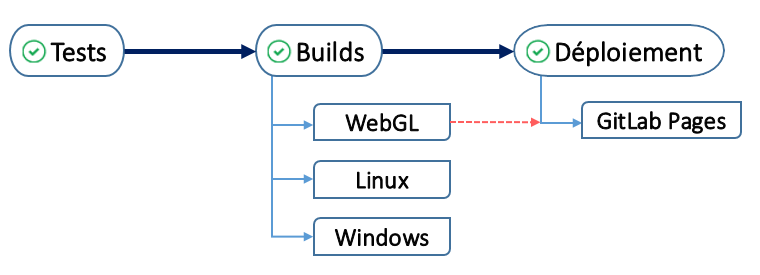
\includegraphics[width=10cm]{IC-DC.png}
    \end{center}
    \caption{Le devops sur Gitlab}
\label{DevopsGitlab}
\end{figure}


Afin de mettre en place l'environnement de Devops, \emph{Sylvain Maurin}, l'administrateur réseau de l'\gls{isc} nous a mis a disposition en plus de notre poste de travail 3 serveurs.
Sur le premier, nous avons installé notre Gitlab. C'est notre Master. Nous avons décidé d'utiliser les deux autres serveurs comme des runners qui, selon la demande du serveur Master
vont réaliser les tests et faire les builds. Comme nous avons décidé de réaliser plusieurs builds (WebGL, Linux et Windows), les runners peuvent
créer les builds en parallèle.

\newpage
\paragraph{Chaine de production}Le schéma suivant montre la chaine de production, de la modification du code jusqu'à l'utilisation de notre jeu par le client :
\begin{itemize}
\item Le développeur pousse ses modifications sur Gitlab
\item Gitlab lance la procédure d'intégration continue
\item Les deux runners exécutent les test unitaires
\item Si les tests passent, ils créent les builds et les retournent au Gitlab
\item Des que Gitlab possède tous les builds, il déploie le jeu sur Gitlab Pages
\item Le client peut jouer à notre jeu sur navigateur à l'adresse du Gitlab Pages
\end{itemize}


\begin{figure}[H]
    \begin{center}
    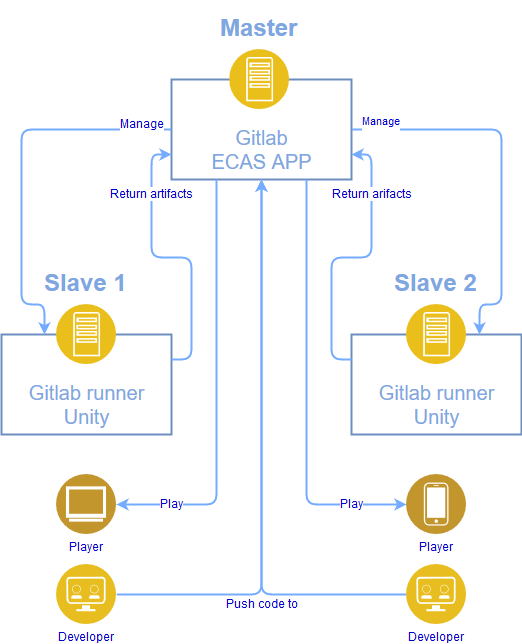
\includegraphics[width=10cm]{network_schema.png}
    \end{center}
    \caption{Schéma du réseau}
\label{NetworkSchema}
\end{figure}